\chapter{Vorauslegung}
\label{chap:Vorauslegung}
% Ziel hier: den Leser in die Lage versetzen, die wesentliche Struktur der Arbeit nachvollziehen zu können (Vorgehen / Geräte / Materialien / Verfahren [also auch Software]  / getroffene Annahmen ... sollten hier erklärt werden)
Die Flugdaten kommen aus einer Trajektoriensimulation aus dem Simulationsprogramm OpenRocket, welche vom Triebwerk-Subsystem durchgeführt wurde.
Diese Flugdaten~(\ref{fig:flugdaten_trajektoriensimulation}) bilden eine Maximalabschätzung der Aerodynamischen Aufheizung und Flugdauer durch
maximale Schubkraft und Dauer mit \SI{8}{\kilo\newton} für \SI{43}{\second}, die von \ac{blast} erreicht werden können.

\section{Anforderungen}

Da die Kühlung zeitgleich zu der Avionik entwickelt wurde, musste auf eine genaue Analyse aller Komponenten der Avionik verzichtet werden.
Stattdessen wurde anhand des bereits festgelegten Microcontrollers STM32H743ZGT6, der auf den redundanten Flugcomputern verwendet wird,
die Auslegung durchgeführt.
Aus dem Datenblatt des Microcontrollers folg eine maximale Sperrschichttemperatur von $T_\text{J} = \SI{125}{\degreeCelsius}$~\cite{STM32}
und ein Sperrschicht-Gehäuse Wärmeleitwiederstand von $\Theta_\text{JC} = \SI{23.9}{\degreeCelsius\per\watt}$~\cite{STM32}. Mit einem konservativen
Sicherheitsfaktor von 1.5, um bisher unbekannte Bauteile zu berücksichtigen, folgt daraus $\Theta_\text{JC,safety} = \SI{35.85}{\degreeCelsius\per\watt}$
und eine maximale Gehäusetemperatur von $T_\text{C} = \SI{89.15}{\degreeCelsius}$. Im Kontext der Elektronik ist mit Gehäuse immer die
Oberseite der elektronischen Komponente gemeint.
Die Kühlung soll außerdem eine hohe Zuverlässigkeit haben, welche durch Verwendung von ausschließlich passiven Bauteilen gewehrleistet wird.
Dadurch kann aufwendiges und teures testen und verifizieren von aktiven Bauteilen mit mechanischer oder elektrischer Funktion vermieden werden und es besteht bei
nicht nominalen Flügen eine geringere Ausfallwahrscheinlichkeit durch die inherent größeren Toleranzen passiver Bauteile.

Dem Energieerhaltungssatz nach haben der \ac{fcc}, die Kameras und weitere Elektronik die keine Leistung abgibt, gegenüber etwa
der \ac{pcdu} und Funkplatine welche Leistung in Form von Strom und elektromagnetischer Strahlung abgeben, einen Wirkungsgrad von
\SI{0}{\percent}, da Logikoperationen physikalisch gesehen keine Arbeit sind. Resultierend wird der komplette Stromverbrauch
in Wärme umgewandelt.

\begin{table}[H]
  \centering
  \caption{Leistung der Avionik}\label{tab:avionik_leistung}

  \begin{tabular}{lp{4cm}ll}
    \toprule[1pt]
    Komponente & Spannung \& Strom & Wirkungsgrad & Wärmestrom \\
    \midrule[0.5pt]

    STM32H743ZGT6 &
      \mbox{$V_\text{DD}=\SI{3.3}{\volt}$},\newline
      $I_\text{DD}=\SI{536}{\milli\ampere}$~\cite{STM32} &
      $\approx \SI{0}{\percent}$ & \SI{1.769}{\watt} \\
    $\dot{Q}_\text{ges}$ & & & \SI{7.075}{\watt}\\

    \midrule[0.5pt]
    RunCam Split 4 V2 &
      \mbox{$V_\text{DD}=\SI{5}{\volt}$},\newline
      $I_\text{DD}=\SI{450}{\milli\ampere}$~\cite{RunCam-Split4V2} &
      $\approx \SI{0}{\percent}$ & \SI{2.25}{\watt} \\
    $\dot{Q}_\text{ges}$ & & & \SI{9}{\watt}\\

    \midrule[0.5pt]
    Thebe-II &
      \mbox{$V_\text{DD}=\SI{3.6}{\volt}$},\newline
      $I_\text{DD}=\SI{500}{\milli\ampere}$~\cite{WE-ThebeII-UM-2024} &
      $\approx \SI{30}{\percent}$~\cite{WE-ThebeII-UM-2024} & \SI{1.3}{\watt} \\

    \midrule[0.5pt]
    \ac{pcdu} & & $\approx \SI{30}{\percent}$ & \SI{9.3}{\watt} \\

    \midrule[0.5pt]
    \midrule[0.5pt]
    $\dot{Q}_\text{ges, safety}$ & & & \SI{40}{\watt} \\

    \bottomrule[1pt]
  \end{tabular}
\end{table}

Die Leistung der Avionik in~\ref{tab:avionik_leistung} ergibt sich durch den Maximalverbrauch der \ac{fcc} mikrocontroller
(STM32H743ZGT6) bei maximaler clock rate (\SI{400}{\mega\hertz}) und vollständig aktiver Peripherie, der Kameras und einer
Abschätzung der restlichen Komponenten ohne Quellenangabe. Der aus \ref{tab:avionik_leistung} resultierende gesamten Wärmestrom
der Avionik mit \SI{40}{\watt} ist mit einem gewöhnlichen Laptop vergleichbar.

\begin{figure}[H]
    \centering

    % Column 1, Row 1
    \begin{subfigure}{0.48\textwidth}
        \centering
        \includegraphics[width=\linewidth]{../../Code/acceleration_over_time.pdf}
        \caption{Beschleunigung während Flug}
        \label{fig:acceleration_over_time}
    \end{subfigure}
    \hfill
    % Column 2, Row 1
    \begin{subfigure}{0.48\textwidth}
        \centering
        \includegraphics[width=\linewidth]{../../Code/altitude_over_time.pdf}
        \caption{Flughöhe}
        \label{fig:altitude_over_time}
    \end{subfigure}

    \vspace{1em}

    % Column 1, Row 2
    \begin{subfigure}{0.48\textwidth}
        \centering
        \includegraphics[width=\linewidth]{../../Code/pressure_over_time.pdf}
        \caption{Statischer Luftdruck während Flug}
        \label{fig:pressure_over_time}
    \end{subfigure}
    \hfill
    % Column 2, Row 2
    \begin{subfigure}{0.48\textwidth}
        \centering
        \includegraphics[width=\linewidth]{../../Code/temperature_over_time.pdf}
        \caption{Statische Lufttemperatur während Flug}
        \label{fig:temperature_over_time}
    \end{subfigure}

    \vspace{1em}

    % Column 1, Row 3
    \begin{subfigure}{0.48\textwidth}
        \centering
        \includegraphics[width=\linewidth]{../../Code/velocity_over_time.pdf}
        \caption{Geschwindigkeit während Flug}
        \label{fig:velocity_over_time}
    \end{subfigure}
    \hfill
    % Column 2, Row 3
    \begin{subfigure}{0.48\textwidth}
        \centering
        \includegraphics[width=\linewidth]{../../Code/dynp_during_flight.pdf}
        \caption{Dynamischer Druck während Flug}
        \label{fig:dynp_over_time}
    \end{subfigure}

    \caption{Flugdaten der Trajektoriensimulation}\label{fig:flugdaten_trajektoriensimulation}
\end{figure}

\section{Thermale Schnittstelle}\label{sec:thermale_schnittstelle}

Um mit der Abwärme der Avionik umgehen zu können, muss sie effektiv gesammelt und abtransportiert werden.
Oft wird in der Luft- und Raumfahrtindustrie Kühlkreisläufe mit einem Arbeitsfluid verwendet. Diese benötigen jedoch
meist bewegliche Bauteile wie Pumpen, welche die Ausfallwahrscheinlichkeit erhöhen. Alternativ gibt es auch
Möglichkeiten durch erzwungene Konvektion ein Arbeitsfluid anzutreiben oder Materialien mit hoher Wärmeleitfähigkeit
zu verwenden. Beide Methoden bieten in Kombination eine günstige Integrierbarkeit und geringen Wärmeleitwiederstand,
ohne Bewegliche Teile zu verwenden.

Das Thermale Interface wird auf Systemebene analysiert, da eine Entwicklung auf \ac{pcb} Ebene wie bereits erläutert nicht
möglich ist, ohne vollständig entwickelte Elektronik.

\subsection{Heatpipes}\label{sec:waermerohre}

Heatpipes (Wärmerohre) sind eine Möglichkeit durch erzwungene Konvektion Wärme zu transportieren. Reguläre Heatpipes
sind vollständig geschlossene Rohre mit einer Flüssigkeit im inneren und einer Kapillarstruktur an der Innenwand,
so dass ein freier Kanal in der Mitte bleibt. Bei der Wärmequelle
verdampft die Flüssigkeit aus der Kapillarstruktur und bei der Wärmesenke kondensiert es wieder, wodurch der resultierende Massenstrom einen
Kreislauf bildet. Besonders effektiv sind Heatpipes durch die Nutzung der Verdampfungsenthalpie beim Flüssig-Gas Übergang an der Wärmequelle,
wodurch sehr hohe Wärmestromdichten erreicht werden können. Eine Schematische Darstellung eines Wärmerohrs kann in \ref{fig:waermerohr}
gesehen werden.

Eine Weiterentwicklung davon sind Loop Heatpipes die, wie der Namen bereits impliziert einen Kreislauf bilden, indem es eine
separate Flüssig- und Dampfleitung gibt, welche jeweils am Verdampfer bzw. Kondensator miteinander verbunden ist.
Besonders von Vorteil sind Loop Heatpipes, wenn größere Distanzen überbrückt werden müssen, oder eine relativ zuverlässige
Funktion unabhängig von Orientierung und Gravitation gebraucht wird. Aufgrund der erhöhten Komplexität von Loop Heatpipes, der Möglichkeit
die Orientierung frei zu bestimmen, den relativ geringen Distanzen innerhalb der Avionik-sektion und dem Mangel an Kommerziell erhältlichen
Loop Heatpipes wird eine reguläre Heatpipe gewählt.


\begin{figure}[H]
  \centering
  \begin{tikzpicture}
    \draw[thick] (-5,0) arc [start angle=90, end angle=270, x radius=1.5cm, y radius= 1.5cm]; % Kappen
    \draw[thick] (5,0) arc [start angle=90, end angle=-90, x radius=1.5cm, y radius= 1.5cm];

    \draw[thick] (-5,0) -- (5,0); % hülle
    \draw[thick] (-5,-3) -- (5,-3);

    \draw[dashed] (-5,0) rectangle (5,-1); % Wick Abgrenzung
    \draw[dashed] (-5,-2) rectangle (5,-3);

    \draw[->, thick, -{Stealth[length=0.25cm]}] (-1,-1.75) -- node [midway, above] {Dampfstrom} (1,-1.75); % Dampf Pfeil
    \draw[->, thick, -{Stealth[length=0.25cm]}] (1,-2.75) -- node [midway, above] {Flüssigstrom}(-1,-2.75); % Flüssigkeitspfeil
    \draw[->, thick, -{Stealth[length=0.25cm]}] (1,-0.5) -- (-1,-0.5); % Flüssigkeitspfeil

    \node at (-4,-4) [style={single arrow, draw}, minimum height=0.5cm, minimum width=1.5cm, shape border rotate=90, thick]{$\dot{Q}$}; % Wärmestrom pfeil
    \node at (4,-3.75) [style={single arrow, draw}, minimum height=0.5cm, minimum width=1.5cm, shape border rotate=270, thick]{$\dot{Q}$}; % Wärmestrom pfeil
    
    \draw[->, thick, -{Stealth[length=0.25cm]}] (-4,0.25) node [above=1pt] {Kapillarstruktur} -- (-3,-0.5); % Kapillar Pfeil
    \draw[->, thick, -{Stealth[length=0.25cm]}] (-4,0.25) -- (-3,-2.5);
  \end{tikzpicture}
  \caption{Wärmerohr Aufbau und Funktionsweise}\label{fig:waermerohr}
\end{figure}

Ein wichtiger Aspekt von Heatpipes ist, dass der Wärmeleitwiederstand durch Biegungen und Anbindung von mehreren Quellen um bis zu \SI{100}{\percent}
steigen kann \cite{Mooney-2020}. Des weiteren hängt besonders bei regulären Heatpipes der Wärmeleitwiederstand von der effektiven Beschleunigung ab,
da die höhere Dichte der Flüssigphase eine beschleunigende Wirkung auf die Konvektion hat, wenn die Wärmequelle unten orientiert ist. Sollte die Heatpipe jedoch
\glqq überkopf \grqq{} arbeiten, sodass die Wärmequelle oben orientiert ist, muss die Konvektion gegen die Beschleunigung arbeiten und verliert Leistung bzw. hat
einen erhöhten Wärmeleitwiederstand.

Ausgewählt wurde die QG-SHP-D5-400MN Heatpipe von Quick-Ohm Küpper \& Co. GmbH aus Kupfer mit Mesh-Gewebe als Kapillarstruktur von \SI{400}{\milli\meter} Länge und
\SI{5}{\milli\meter} Durchmesser. Diese Heatpipe kann eine Leistung von \SI{40}{\watt} übertragen und hat einen angegebenen Wärmeleitwiederstand
von \SI{0,3}{\kelvin\per\watt}

Weiterhin wird die Heatpipe als \ac{rom} mit einem einfachen Widerstand ersetzt, der dem Wärmeleitwiederstand der Heatpipe aus dem Datenblatt~\cite{QuickOhm-Heatpipe-5x400} entspricht.

\subsection{Wärmeleitbänder}\label{sec:waermebaender}

Um die Elektronik mit dem Wärmerohr zu verbinden werden Wärmeleitbänder aus verschiedenen Materialien analysiert.
Wärmeleitbänder sind flexible Verbindungsteile mit hoher Wärmeleitfähigkeit die Wärmebrücken zwischen mehreren Bauteilen gewährleisten.
\ac{pgs} ist gegenüber herkömmlichen Materialien besonders interessant durch die extrem hohe Wärmeleitfähigkeit innerhalb der Ebene,
da diese der Ebene von der Molekülstruktur des Graphit entspricht. Außerdem ist es ein relativ flexibles Material, bei einer üblichen Dicke von $\approx \SIrange{10}{100}{\micro\meter}$.
Ein Nachteil von \ac{pgs} ist die im Kontrast zur Ebene sehr niedrige Wärmeleitfähigkeit durch die Ebene, infolge von wenigen
molekularen Brücken zwischen den Gitterstrukturen. Dementsprechend wird \ac{pgs} und andere Arten von Graphit Folien hauptsächlich zur
Wärmeverteilung auf der Oberfläche von Bauteilen verwendet um Wärmestromdichten zu verringern und homogenere Temperaturverteilungen zu erreichen.

Das effektive erhöhen des Querschnitts von \ac{pgs} durch Schichtung mehrerer Folien aufeinander ermöglicht es jedoch die hohe
Wärmeleitfähigkeit in der Ebene auch zum thermischen koppeln mehrerer Bauteile zu verwenden. Diese Anwendung hat besonders in der 
Raumfahrt durch ermöglichte Masseneinsparungen Halt gefunden. Eine Kommerzielle Reihe an solchen Wärmeleitbändern aus gängigen Materialien sieht man in~\ref{fig:thermalstraps_commercial}.
Der Tabelle~\ref{tab:strap_materials} nach ist \ac{pgs} das beste Kompromiss für die geforderten Eigenschaften und wurde für die weitere Analyse ausgewählt.

\begin{figure}[H]
  \centering
  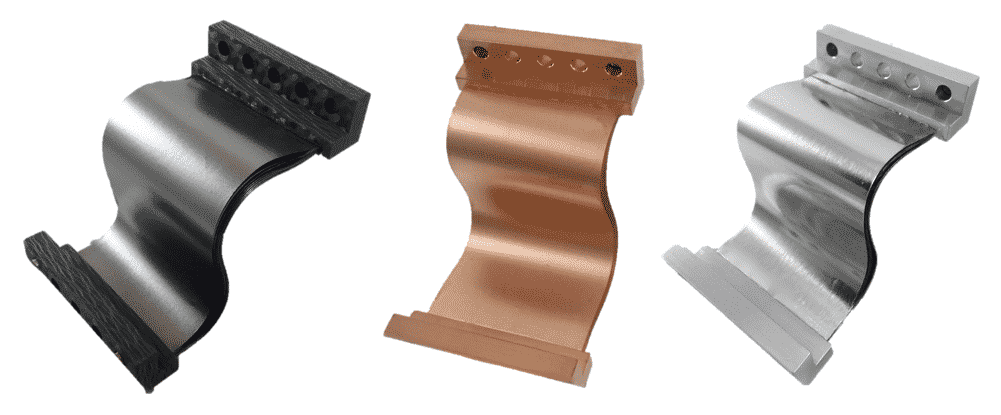
\includegraphics[width=\textwidth]{thermal_straps_commercial.png}
  \caption{Kommerziell erhältliche Wärmeleitbänder aus Graphen (links), Kupfer und Aluminium~\cite{Thermal-Straps}}\label{fig:thermalstraps_commercial}
\end{figure}

Aufgrund der höchsten Wärmeleitfähigkeit in der Ebene vom \ac{pgs} HGS-012 der Firma HPMS Graphite wurde dieses ausgewählte.


\definecolor{good}{RGB}{200,255,200}   % hellgrün
\definecolor{medium}{RGB}{255,255,200} % hellgelb
\definecolor{bad}{RGB}{255,200,200}    % hellrot

\begin{table}[H]
  \centering
  \caption{Ampelbewertung von Materialien für Wärmeleitbänder. Rot entspricht schlechten Eigenschaften, grün guten und gelb dem Wert dazwischen.}\label{tab:strap_materials}

  % 1. Spalte als Box-Spalte, damit \\ innerhalb der ZELLE umbricht
  \begin{tabular}{>{\raggedright\arraybackslash}m{3cm} m{3.2cm} m{3.2cm} m{3cm}}
    \toprule[1pt]
    Eigenschaft & Kupfer\cite{Thermtest-DB} & Aluminium\cite{Thermtest-DB} & PGS \nobreak{(Graphit)}\cite{HPMS-PGS} \\
    \midrule[0.5pt]

    \makecell[l]{Wärmeleit-\\fähigkeit\\in Ebene}
      & \cellcolor{medium}\SI{397.48}{\watt\per\meter\per\kelvin}
      & \cellcolor{bad}\SI{225.94}{\watt\per\meter\per\kelvin}
      & \cellcolor{good}\SIrange{1050}{1800}{\watt\per\meter\per\kelvin} \\

    \makecell[l]{Wärmeleit-\\fähigkeit\\durch Ebene}
      & \cellcolor{good}\SI{397.48}{\watt\per\meter\per\kelvin}
      & \cellcolor{medium}\SI{225.94}{\watt\per\meter\per\kelvin}
      & \cellcolor{bad}\SIrange{10}{26}{\watt\per\meter\per\kelvin} \\

    Dichte
      & \cellcolor{bad}\SI{8940}{\kilogram\per\cubic\meter}
      & \cellcolor{medium}\SI{2698}{\kilogram\per\cubic\meter}
      & \cellcolor{good}\SIrange{1500}{2100}{\kilogram\per\cubic\meter} \\

    Elektrische \makecell[l]{\\Isolation}
      & \cellcolor{bad}Schlecht
      & \cellcolor{bad}Schlecht
      & \cellcolor{bad}Schlecht \\
    \bottomrule[1pt]
  \end{tabular}
\end{table}

Mittels einer Kombination von \ac{pgs} und Heatpipe kann eine leicht integrierbare Wärmebrücke gebildet werden, die den Wärmeleitwiederstand
minimiert. Eine Schematische Darstellung der Thermalen Schnittstelle 

\begin{figure}[H]
  \centering
  \begin{tikzpicture}
    \node at (0,0) [style={single arrow, draw}, minimum height=0.5cm, minimum width=1.5cm, shape border rotate=90, thick]{$\dot{Q}$}; % Wärmestrom pfeil

    \draw[thick] (0,-1) -- (0,-3.1);

    \draw[thick] (0,-3.1) -- (-0.2,-3.2); % heatpipe resistor
    \draw[thick] (-0.2,-3.2) -- (0.2,-3.4);
    \draw[thick] (0.2,-3.4) -- (-0.2,-3.6);
    \draw[thick] (-0.2,-3.6) -- (0.2,-3.8);
    \draw[thick] (0.2,-3.8) -- (-0.2,-4);
    \draw[thick] (-0.2,-4) -- (0.2,-4.2);
    \draw[thick] (0.2,-4.2) -- (0,-4.3);

    \node[rotate=90] at (-0.5,-3.7) {Heatpipe};
    \node at (2.5,-3.7) {$R_{\mathrm{Heatpipe}} = \SI{0,3}{\kelvin\per\watt}$};

    \draw[thick] (0,-4.3) -- (0,-6.4);

    \draw[thick] (0,-6.4) -- (2.1,-6.4);

    \fill (0,-6.4) circle (1.5pt); %knotenpunkt

    \begin{scope}[shift={(-1,-6.4)}, rotate=90]
      \draw[thick] (0,-3.1) -- (-0.2,-3.2); % thermal strap resistor
      \draw[thick] (-0.2,-3.2) -- (0.2,-3.4);
      \draw[thick] (0.2,-3.4) -- (-0.2,-3.6);
      \draw[thick] (-0.2,-3.6) -- (0.2,-3.8);
      \draw[thick] (0.2,-3.8) -- (-0.2,-4);
      \draw[thick] (-0.2,-4) -- (0.2,-4.2);
      \draw[thick] (0.2,-4.2) -- (0,-4.3);
    \end{scope}


    \node at (2.7,-5.9) {Wärmeleitband};
    \node at (2.7,-6.9) {$R_{\mathrm{Wärmeleitband}} = \SI{000}{\kelvin\per\watt}$};

    \draw[thick] (3.3,-6.4) -- (5.4,-6.4);

    \node at (6.4,-6.4) [style={single arrow, draw}, minimum height=0.5cm, minimum width=1.5cm, shape border rotate=180, thick]{$\frac{\dot{Q}}{4}$}; % Wärmestrom pfeil

    \draw[thick] (0,-6.4) -- (0,-8.4);

    \draw[thick] (0,-8.4) -- (2.1,-8.4);

    \fill (0,-8.4) circle (1.5pt);% knotenpunkt 2

    \begin{scope}[shift={(-1,-8.4)}, rotate=90]
      \draw[thick] (0,-3.1) -- (-0.2,-3.2); % thermal strap resistor 2
      \draw[thick] (-0.2,-3.2) -- (0.2,-3.4);
      \draw[thick] (0.2,-3.4) -- (-0.2,-3.6);
      \draw[thick] (-0.2,-3.6) -- (0.2,-3.8);
      \draw[thick] (0.2,-3.8) -- (-0.2,-4);
      \draw[thick] (-0.2,-4) -- (0.2,-4.2);
      \draw[thick] (0.2,-4.2) -- (0,-4.3);
    \end{scope}

    \node at (2.7,-7.9) {Wärmeleitband};
    \node at (2.7,-8.9) {$R_{\mathrm{Wärmeleitband}} = \SI{000}{\kelvin\per\watt}$};

    \draw[thick] (3.3,-8.4) -- (5.4,-8.4);

    \node at (6.4,-8.4) [style={single arrow, draw}, minimum height=0.5cm, minimum width=1.5cm, shape border rotate=180, thick]{$\frac{\dot{Q}}{4}$}; % Wärmestrom pfeil

    \draw[thick] (0,-8.4) -- (0,-9);

    \node[rotate=90] at (0,-9.5) {$\cdots$};

    \draw[->, thick, -{Stealth[length=0.25cm]}] (-1.5,-6) -- node [pos=0,above=1pt] {$g$} (-1.5,-8); % Gravitation
  \end{tikzpicture}
  \caption{\ac{rom} der Thermalen Schnittstelle aus Heatpipe und Wärmeleitbändern. Hier sind nur 2 von 4 Wärmeleitbändern dargestellt.}\label{fig:thermale_schnittstelle}
\end{figure}

\section{PCM}

\ac{pcm} mit Fest-Flüssig Übergang ist eine weit verbreitete Lösung in der Luft- und Raumfahrtindustrie um für für begrenzte Zeiträume Elektronik in einem akzeptablen
Temperaturbereich zu halten. Auch wenn \ac{pcm} Lösungen generell eine hohe Masse haben, wird das oft aufgrund der ansonsten idealen Eigenschaften inkauf genommen.
Durch die hohe spezifische Schmelzenthalpie, kann rein passiv eine große Wärmemenge, bei einem isothermen Prozess, absorbiert werden. Aufgrund dessen
kann ein von der Umwelt isoliertes \ac{atm} entwickelt werden, das nicht mit stark schwankenden Zuständen der Sonneneinstrahlung und Lufttemperatur
zurecht kommen muss. Auch wenn \ac{pcm} im Flüssig-Gas Übergang meist eine etwa 10-fach höhere Verdampfungsenthalpie haben, werden diese
generell nicht verwendet, da der Dichteunterschied zwischen Flüssig- und Gasphase zu extremen Drücken führen würden, falls Wiederverwendbarkeit
verlangt wird und somit ein Druckkörper nötig ist. Alternativ kann die Gasphase auch aus dem Fahrzeug abgelassen werden in einem Prozess der
Vapour Venting genannt wird. Hierbei geht jedoch die Wiederverwendbarkeit verloren, da vor jedem Start die Flüssigphase neu getankt werden muss.
Weiter kann das Venting trotz der geringen Massenströme zu Momenten führen, die das Fahrzeug destabilisieren; besonders im Überschallbereich
können unintuitive Momente entstehen~\cite{Deere-2011}, die aufwendige \ac{cfd}-Simulationen oder Tests benötigen. Dementsprechend wird nur ein
Fest-Flüssig \ac{pcm} analysiert.\\

Für die Auswahl eines geeigneten \ac{pcm} sind spezifische Schmelzenthalpie, Schmelztemperatur und Wärmeleitfähigkeit am wichtigsten.
Letzteres kann jedoch durch Lamellen oder ähnliche Strukturen, zur Verbesserung der Wärmeleitfähigkeit durch das komplette \ac{pcm} verbessert werden,
wobei dabei \ac{pcm} Masse mit Strukturmasse ersetzt wird und somit die Wärmekapazität verringert. Das Volumen der Wärmeleitenden Struktur welches
\ac{pcm} ersetzt wird Void Fraction genannt, da es gewissermaßen eine Leerstelle im \ac{pcm} bildet, die keine latente Wärmeaufnahme hat. Hier
wird ein Void Fraction von $F = 0.1$ todo

Die Thermodynamischen Eigenschaften von Eicosane, aufgeführt in Tabelle \ref{tab:eicosane_data}, wurden aus mehreren Quellen entnommen.
Vor der Implementierung des \ac{pcm} sollten die Eigenschaften des vorhandenen Eicosane nochmal analysiert und die Ergebnisse überprüft werden.

\begin{table}[H]

  \centering
  \caption{Stoffdaten für Eicosane}\label{tab:eicosane_data}

  \begin{tabular}{lll}

    \toprule[1pt]
    Solidus Temperatur & $T_{\text{solidus}}$ & \SI{309}{\kelvin}~\cite{NIST} \\

    \midrule[0.5pt]
    Liquidus Temperatur & $T_{\text{liquidus}}$ & \SI{311}{\kelvin}~\cite{NIST} \\

    \midrule[0.5pt]
    Spezifische Wärmekapazität bei\\konstantem Druck der\\Flüssigphase & $c_{p,\text{liquid}}$ & \SI{2350.05}{\joule\per\kilogram\per\kelvin}~\cite{NIST} \\

    \midrule[0.5pt]
    Spezifische Wärmekapazität bei\\konstantem Druck der\\Feststoffphase & $c_{p,\text{solid}}$ & \SI{2132.4}{\joule\per\kilogram\per\kelvin}~\cite{NIST} \\

    \midrule[0.5pt]
    Dichte der Flüssigphase & $\rho_{\text{solid}}$ & \SI{910}{\kilogram\per\cubic\meter}~\cite{Nazarychev-2022} \\

    \midrule[0.5pt]
    Dichte der Feststoffphase & $\rho_{\text{liquid}}$ & \SI{769}{\kilogram\per\cubic\meter}~\cite{Nazarychev-2022} \\

    \midrule[0.5pt]
    Wärmeleitfähigkeit der Flüssigphase & $\lambda_{\text{liquid}}$ & \SI{0.1505}{\watt\per\meter\per\kelvin}~\cite{Benbrika-2020} \\

    \midrule[0.5pt]
    Wärmeleitfähigkeit der Feststoffphase & $\lambda_{\text{solid}}$ & \SI{0.4248}{\watt\per\meter\per\kelvin}~\cite{Stryker-1990} \\

    \midrule[0.5pt]
    Wärmeausdehnungskoeffizient & $\beta$ & \SI{0.0009}{\per\kelvin}~\cite{Benbrika-2020} \\

    \midrule[0.5pt]
    Spezifische Schmelzenthalpie & $h_{\text{fus}}$ & \SI{240998.86}{\joule\per\kilogram}~\cite{NIST} \\

    \bottomrule[1pt]
  \end{tabular}
\end{table}

\begin{lstlisting}[float, language=Python, caption={Berechnung der Masse und Latenten Wärmekapazität des \ac{pcm} in der pcm.py}, label={lst:pcm_masse_kapazität}]
rho_alu = 2700     # aluminium density [kg*m^-3]
rho_pcm = 788      # pcm density [kg*m^-3]
h      = 240998.9  # pcm latent heat [J*kg^-1]
F       = 0.1      # void fraction
t       = 0.001    # wall thickness [m]

def total_mass(L, H): # pcm mass including case and fins
    return (rho_alu * (L**2 * H - (L - 2*t)**2 * (H - 2*t))
            + (F * rho_alu + (1 - F) * rho_pcm) * (L - 2*t)**2 * (H - 2*t)) 

def total_heat(L, H): # pcm latent heat capacity
    #...#
    pcm_heat  = (1 - F) * rho_pcm * (L - 2*t)**2 * (H - 2*t) * h
    return pcm_heat
\end{lstlisting}

Die pcm masse und kapazität kontour sieht man im anhang

\newpage

\section{Radiator}\label{sec:Radiator}

Bei Radiatoren ist ein hoher Emissions- und niedriger Absorptionsgrad nach \ref{eq:radiation} dimensionierend, da die Temperatur den Anforderungen nach limitiert ist
und die Fläche minimiert werden muss, da diese proportional zu eingehende Wärmeströmen aus der Umgebung ist, welche auch möglichst gering gehalten werden müssen.\\
Als Beschichtung wurde AZ-93 der Firma AZ Technology LLC.~\cite{AZ-Technology} ausgewählt. Dabei handelt es sich um eine in der Raumfahrt
weit verbreitete inorganische Farbe mit idealen Eigenschaften, welche Tabelle \ref{tab:az-93_eigenschaften} entnommen werden können.
In \ref{fig:radiator_flaeche_leistung} sieht man für die ausgewählte Beschichtung die Leistung eines Radiators bei gegebener Temperatur und Fläche.
Durch in \ref{sec:pcm_radiator_hybrid} analysierte Wärmeströme, würde es bei nutzung eines einfachen Radiators schnell zur Überhitzung der Avionik kommen.\\


\begin{table}[H]

  \centering
  \caption{AZ-93 Spezifikationen~\cite{AZ-Technology}}\label{tab:az-93_eigenschaften}

  \begin{tabular}{ll}

    \toprule[1pt]
    $\varepsilon_{\text{t}}$ & $0.91 \pm 0.02$ \\

    \midrule[0.5pt]
    $\alpha_{\text{s}}$ & $0.15 \pm 0.02$ \\

    \midrule[0.5pt]
    Temperaturbereich  & \SI{-180}{\degreeCelsius} bis \SI{1400}{\degreeCelsius} \\

    \bottomrule[1pt]
  \end{tabular}
\end{table}

Die konturen des Radiators können im Anhang gefunden werden

\newpage

\section{PCM-Radiator-Hybrid}\label{sec:pcm_radiator_hybrid}

Eine Hybridlösung wird auch in erwägung gezogen, um die Masse durch Nutzung eines Radiators zu minimieren, wobei wegen aerodynamischer Aufheizung für kurze Zeit ein PCM gebraucht werden könnte.
Um eine umständliche Simulation mittels \ac{cfd} zu vermeiden, wird die Außenkontour der Rakete von Spitze bis Avionik-Sektion, mit Hilfe der Nußelt-Beziehungen, als längsangeströmte ebene Platte angesehen,
wie in Abbildung~\ref{fig:rakete_kontour_zeichnung} dargestellt ist.
Um zu wissen, ob hier die Beziehung für laminare oder turbulente Grenzschichten angewandt werden soll, müssen zunächst die Gültigkeitsbereiche der Reynolds- und Prandtlzahl (\ref{eq:prandtl},~\ref{eq:reynolds}) überprüft werden.
Mittels der Nußelt-Beziehung wird $\alpha$ bestimmt und dann in Gleichung~\ref{eq:qdot} eingesetzt, um auf den spezifischen Wärmestrom zu schließen.

\newpage
% Hybrid PCM ohne aufheizung

\begin{figure}
  \centering
  \begin{tikzpicture}[rotate border/.style={shape border uses incircle, shape border rotate=#1}, scale=0.8]
    \draw[thick] (3,3) -- (3,-1) -- (9,-1) -- (9,3);
    \draw[thick] (3,3) -- node [midway, above] {Avionik Sektion}  (9,3);
    \draw[thick] (4,3) -- (4,-1); % PCM Lamellen
    \draw[thick] (3,-0.5) -- (4,-0.5);
    \draw[thick] (3,0) -- (4,0);
    \draw[thick] (3,0.5) -- (4,0.5);
    \draw[thick] (3,1) -- (4,1);
    \draw[thick] (3,1.5) -- (4,1.5);
    \draw[thick] (3,2) -- (4,2);
    \draw[thick] (3,2.5) -- (4,2.5);
    \node at (-0.5,2) [style={single arrow, draw}, minimum height=3cm, minimum width=0.5cm, thick]{$\dot{Q}_{\mathrm{Umwelt}}$}; % Wärmestrom pfeil
    \node at (-0.5,0) [style={single arrow, draw}, minimum height=4.5cm, minimum width=1.5cm, shape border rotate=180, thick]{$\dot{Q}_{\mathrm{Radiator}}$}; % Wärmestrom pfeil
    \node at (6.5,1)[style={single arrow, draw}, minimum height=3cm, minimum width=0.5cm, shape border rotate=180, thick]{$\dot{Q}_{\mathrm{Avionik}}$}; % Wärmestrom pfeil
    \draw[->, thick, -{Stealth[length=0.25cm]}] (1,3.75) node [above=1pt] {PCM mit Lamellen} -- (3.5,2.6);
  \end{tikzpicture}
  \caption{PCM Wärmestrom ohne aerodynamische Aufheizung}\label{fig:pcm_waermestrom_diagramm}
\end{figure}

$\dot{Q}_{\mathrm{Radiator}} = \dot{Q}_{\mathrm{Umwelt}} + \dot{Q}_{\mathrm{Avionik}}$ In diesem Fall reicht die Leistung des Radiators, um die Avionik auf Betriebstemperatur zu halten.
% Hybrid PCM Wärmestrom bei aufheizung

\begin{figure}[H]
  \centering
  \begin{tikzpicture}[rotate border/.style={shape border uses incircle, shape border rotate=#1}, scale=0.8]
    \draw[thick] (3,3) -- (3,-1) -- (9,-1) -- (9,3);
    \draw[thick] (3,3) -- node [midway, above] {Avionik Sektion}  (9,3);
    \draw[thick] (4,3) -- (4,-1); % PCM lamellen
    \draw[thick] (3,-0.5) -- (4,-0.5);
    \draw[thick] (3,0) -- (4,0);
    \draw[thick] (3,0.5) -- (4,0.5);
    \draw[thick] (3,1) -- (4,1);
    \draw[thick] (3,1.5) -- (4,1.5);
    \draw[thick] (3,2) -- (4,2);
    \draw[thick] (3,2.5) -- (4,2.5);
    \node at (-0.5,2) [style={single arrow, draw}, minimum height=4.5cm, minimum width=1.5cm, thick]{$\dot{Q}_{\mathrm{Umgebung}}$}; % Wärmestrom pfeil
    \node at (-0.5,0) [style={single arrow, draw}, minimum height=4.5cm, minimum width=1.5cm, shape border rotate=180, thick]{$\dot{Q}_{\mathrm{Radiator}}$}; % Wärmestrom pfeil
    \node at (6.5,1)[style={single arrow, draw}, minimum height=3cm, minimum width=0.5cm, shape border rotate=180, thick]{$\dot{Q}_{\mathrm{Avionik}}$}; % Wärmestrom pfeil
  \end{tikzpicture}
  \caption{PCM Wärmestrom bei aerodynamischer Aufheizung}\label{fig:pcm_waermestrom_aufheizung_diagramm}
\end{figure}

Hier reicht die Leistung des Radiators nicht mehr aus und das \ac{pcm} fängt an zu schmilzen. Zu beachten ist,
dass die Leistung des Radiators durch die Temperaturerhöhung steigen würde, wegen des \ac{pcm} jedoch sehen wir das System als isotherm an.
% Raketenkontour im Luftstrom für ebene Platte Annahme

\begin{figure}[H]
  \centering
  \begin{tikzpicture}
    \draw[thick] (0,0) arc [start angle=90, end angle=270, x radius=5cm, y radius= 1.5cm]; %nosecone
    \draw[thick] (0,0) -- (3,0); % hülle
    \draw[thick] (0,-3) -- (3,-3); % hülle
    \draw[thick] (-5.75,-1.5) -- (-5.25,-1.5); % maß links
    \draw[thick] (1,0.25) -- (1,0.75); % maß rechts
    \draw[thick] (0,0.5) arc [start angle=90, end angle=180, x radius=5.5cm, y radius= 2cm]; % maß bogen
    \draw[thick] (0,0.5) -- node [near start, above] {Länge} (1,0.5); % maß grade sektion
    \draw[->, thick, -{Stealth[length=0.25cm]}] (-10,0.5) -- node [midway, above] {Luftstrom} (-7,0.5); % free stream pfeile
    \draw[->, thick, -{Stealth[length=0.25cm]}] (-10,-0.5) -- (-7,-0.5); % Strompfeile
    \draw[->, thick, -{Stealth[length=0.25cm]}] (-10,-1.5) -- (-7,-1.5);
    \draw[->, thick, -{Stealth[length=0.25cm]}] (-10,-2.5) -- (-7,-2.5);
    \draw[->, thick, -{Stealth[length=0.25cm]}] (-10,-3.5) -- (-7,-3.5);
    \draw[thick] (0,0) -- (0,-2.5); % casing wall
    \draw[thick] (2,0) -- (2,-2.5); % casing wall
    \draw[thick] (0,-2.5) -- (2,-2.5); % casing bottom
    \node at (1,-1.5) [style={single arrow, draw}, minimum height=0.5cm, minimum width=1.5cm, rotate=90, thick]{$\dot{Q}_{\mathrm{Avionik}}$}; % Wärmestrom pfeil
  \end{tikzpicture}
  \caption{Kontourlänge vom Staupunkt der Rakete bis zum Mittelpunkt des Radiators}\label{fig:rakete_kontour_zeichnung}
\end{figure}

In Abbildung~\ref{fig:dimensionierung_ablauf} sieht man wie die Dimensionierung in den Programmen abläuft. Die Programme erzeugen alle Graphen und rechnen simultan für gegebenen Avionik Wärmestrom alle Werte aus.

\begin{figure}[H]
  \centering
  \begin{tikzpicture}[
    sibling distance=10em,
    every node/.style = {
      shape=rectangle,
      rounded corners,
      draw,
      align=center,
      minimum width=3cm
    },
    edge from parent/.style = {
      draw,
      ->,
      -{Stealth[length=0.25cm]},
      thick
    },
    arrow/.style = {
      ->,
      -{Stealth[length=0.25cm]},
      thick
    }
  ]

    % Top nodes
    \node (avionik) at (-2.1, 4) {Avionik Wärmestrom};
    \node (sonne)   at ( 2.1, 4) {Solarer Wärmestrom};

    % Radiator Fläche centered below
    \node (radiator) at (0, 2) {Radiator Fläche};

    % Children of Radiator
    \node (breite) at (-2.4, 0) {PCM Breite};
    \node (aerodynamisch) at (2.4, 0) {Aerodynamischer Wärmestrom};

    % PCM Kapazität as a separate node (not a child directly)
    \node (kapazitaet) at (2.1, -2) {PCM Kapazität};

    % PCM Höhe node below the center of breite and kapazitaet
    \node (hoehe) at (0, -4) {PCM Höhe};
    \node (gewicht) at (0, -6) {PCM Gewicht};

    % Arrows
    \draw[arrow] (avionik) -- (radiator);
    \draw[arrow] (sonne) -- (radiator);
    \draw[arrow] (radiator) -- (breite);
    \draw[arrow] (radiator) -- (aerodynamisch);
    \draw[arrow] (aerodynamisch) -- (kapazitaet);
    \draw[arrow] (breite) -- (hoehe);
    \draw[arrow] (kapazitaet) -- (hoehe);
    \draw[arrow] (hoehe) -- (gewicht);

  \end{tikzpicture}
  \caption{Dimensionierungs-Ablauf in der Vorauslegung}\label{fig:dimensionierung_ablauf}
\end{figure}

\begin{figure}[H]
  \centering
  \includegraphics[width=\linewidth]{../../Code/re_pr_during_flight.pdf}\label{fig:re_pr_flugsimulation}
  \caption{Reynolds- und Prandtlzahl während kritischer Phase im Flug}
  \includegraphics[width=\linewidth]{../../Code/pcm_radiator_hybrid_heatflux_nosim.pdf}\label{fig:pcm_waermestrom_vorauslegung}
  \caption{PCM Wärmestrom während Flug}
\end{figure}